\chapter{Konzeption}\label{chapter4}

\section{Vorgehensmodell}
Für dieses Projekt wurde sich für ein inkrementelles, iteratives Wasserfallmodell als Vorgehensmodell entschieden. Zum einen ist dies dadurch begründet, dass Auftraggeber und Projektverantwortlicher die selbe Person sind. Die Projektanforderungen wurden in einem ersten Schritt selbstständig analysiert und definiert. Viele Vorteile eines agilen Modells, zum Beispiel die starke Kommunikation mit dem Kunden gegenüber der kleinteiligen Definition im voraus, sind also garnicht durchführbar. Auch müssen keine Teilartefakte an den Kunden ausgeliefert werden, was in agilen Modellen häufig ein wichtiges Kriterium ist, damit dieser den Fortschritt prüfen kann. Das führt auch dazu, dass sich Anforderungen nicht ändern werden. Trotzdem sind in diesem Projekt einige Unsicherheiten vorhanden und es müssen oft Prototypen angelegt werden, bevor weitere Implementationen geplant werden können. Dies ist der Grund für ein iteratives Vorgehen, bei denen alle Projektphasen nacheinander durchlaufen werden, bevor der Prozess erneut gestartet wird. Die Projektphasen folgen dabei den bekannten, standardisierten Projektphasen.   Als erstes muss an Hand der bereits definierten Anforderungen in der Design-Phase eine Programmiersprache gefunden werden. Anschließend muss die UI geplant werden und die benötigten Bibliotheken evaluiert werden. Auch ist es erforderlich, sich erste Gedanken über die grundlegende Struktur der Anwendung zu machen und eine erste Architektur zu planen. Diese Schritt laufen noch nicht iterativ ab. Immer noch in der Designphase muss jetzt der erste Prototyp geplant werden, wobei hier konkretere Designentscheidungen getroffen werden. Anschließend soll in der Implementierungsphase der Prototyp implementiert werden. Danach muss getestet werden, ob er die Anforderungen erfüllt und evaluiert werden, wie gut er diese erfüllt. Hier sollte auch oft eine Evaluation der User Experience notwendig sein. Die Phasen Design, Implementation, Test und Evaluation werden dann solange wiederholt, bis alle Anforderungen erfüllt wurden. Sollte danach noch genügend Zeit vorhanden sein, kann nach eigenem Ermessen mit der Erfüllung der fakultativen Anforderungen begonnen werden. Auch wenn das Vorgehen hier beschrieben wurde, soll dennoch einem standardisiertem Vorgehen eine geringere Bedeutung zugemessen werden. Auch sind einige Prozesse unnötig, welche normalerweise in diesem Vorgehen durchgeführt werden. Dazu zählt zum Beispiel das Anlegen von Dokumenten zwischen jeder Projektphase, die die Erkenntnisse der vorigen Phase für alle Stakeholder festhalten oder das Durchführen von bestimmten Meetings.

\section{Programmiersprache}
Die Wahl der richtigen Programmiersprache ist mehr als nur reine Präferenz, da jede Sprache projektrelevante Eigenheiten hat. Im folgenden werden daher drei Programmiersprachen auf ihre Projekttauglichkeit evaluiert. Für dieses Projekt irrelevante Aspekte wie zum Beispiel Sprachfeatures oder Paradigmen fließen in die Bewertung nicht mit ein.

Der wichtigste Faktor aus Projektsicht ist das Zielsystem, auf die Software schlussendlich laufen wird. Sie bestimmt schlussendlich über die Zielgruppe und hat einen entscheidenden Einfluss auf die Reichweite des Projekts. Idealerweise sollte es die Sprache erlauben die Software, ohne große Veränderungen, auf eine andere Plattform zu portieren. Hier sind dann Betriebssystem- und Hardware-Unabhängigkeit von großer Bedeutung um dies zu erleichtern. Ein weiterer Aspekt ist die Geschwindigkeit, auch wenn sie einen deutlich kleineren Stellenwert einnimmt, da der Einfluss einer Sprache auf die Gesamtperformance der Anwendung äußerst gering ist und dort wichtigere Aspekte bevorzugt werden sollten\footnote{“premature optimization is the root of all evil” - Sir Tony Hoare}. Ein weiterer wichtiger Punkt ist das Vorhandensein von Tools, welche den Entwicklungsprozess unterstützen können. Hier sind zum Beispiel Debugger, Profiler oder Analyse-Tools zu nennen, mit denen die Performance der Anwendung evaluiert werden kann. Auch das Vorhandensein von Frameworks ist nicht zu unterschätzen, da sie zur Einhaltung des Projektzeitraumes benötigt werden und gerade im Bereich der Grafikprogrammierung nicht für jede Sprache existieren. Schlussendlich müssen auch persönliche Fähigkeiten und Erfahrungen genannt werden. Das Lernen einer neuen Sprache ist zeitintensiv und führt außerdem zu einer erhöhten Fehleranfälligkeit.

\subsection{Java}
Java ist eine objektorientierte Sprache mit sehr hohem Abstraktionsniveau. Sie wird in einer virtuellen Maschine namens Java Virtual Machine (JVM) ausgeführt und ist somit Betriebssystem- und Hardware unabhängig. Dadurch ist das Kriterium der guten Verfügbarkeit erfüllt und eine möglichst große Zielgruppe kann angesprochen werden. Insbesondere Smartphones sind hier als Zielplattform zu erwähnen, da hier die Entwicklung von Apps mit Java favorisiert wird. Auch das Motto “Write Once, Runs Everywhere”, welches sich unter anderem in der Rückwärtskompatibilität bis zur ersten Java Version von vor über 25 Jahren manifestiert, ist für die meisten Softwareprojekte, inklusive diesem, sehr vorteilhaft, da keine Änderungen am Code notwendig sind und die Software weiterhin auf neueren JVMs lauffähig bleibt.

Allerdings beeinträchtigt die Nutzung einer virtuellen Maschine die Nutzung von nativen, also Betriebssystem abhängigen Ressourcen außerhalb dieser isolierten Umgebung, insbesondere den OpenGL Implementationen. Unter anderem verwaltet die JVM jeglichen Speicher, was eine Übergabe von zum Beispiel Speicheradressen (Pointer) von Objekten im Java Heap an OpenGL unmöglich macht. Auch die verfügbaren Referenzen existieren natürlich nur im Kontext der virtuellen Maschine. Als Lösung bietet Java die Nutzung von sogenannten direct buffer an, welche außerhalb der Java Heaps liegen und nicht von der JVM verwaltet werden. Hier ist dann ein ständiges Kopieren zwischen Heap und Buffer notwendig, was vor allem bei der Übergabe großer Vertex Daten problematisch ist. Hier ist viel manuelles Kopieren und das Serialisieren von komplexen Objekten in die Buffer notwendig. Auch die allgemeine Kommunikation mit dem OpenGL Treiber besitzt einen Performance Overhead, der nicht zu vernachlässigen ist.

Aufgrund des Alters der Sprache und seiner hohen Beliebtheit\footnote{seit 2001 in den Top 3 der beliebtesten Sprachen: \url{https://www.tiobe.com/tiobe-index/java/}} existiert ein sehr große Community im Umfeld der Sprache, welcher auch oft als Java Ecosystem beschrieben wird. Dies zeigt sich in einem sehr guten Tooling-Support und einer Implementation der meisten größeren Frameworks in dieser Sprache. Abschließend kann auch die hohe persönliche Expertise mit dieser Sprache als Vorteil genannt werden.

\subsection{C++}
C++ ist eine objektorientierte Sprache mit niedrigerem Abstraktionsniveau als Java. Sie besitzt keine automatische Speicherverwaltung (keine Garbage Collection und explizite Speicher-Allokationen und -Referenzierung). Auch wird sie direkt zu Maschinencode kompiliert und direkt ausgeführt, sodass sie im Allgemeinen als schneller angesehen wird. Die heißt aber auch, dass für jedes Betriebsystem (bzw. sogar für jede CPU) ein eigenes Kompilat erzeugt werden muss. Auch das Web und Smarthphones können nicht ohne weiteres mit dieser Sprache angesprochen werden, was zu einer Verkleinerung der Zielgruppe führt.

Eine kurze Suche nach dem Begriff "OpenGL" in Repositories auf github.com zeigt, dass sie mit Abstand die meistgenutzte Sprache bei der Entwicklung von Grafikanwendungen mit OpenGL ist\footnote{\url{https://github.com/search?q=opengl&type=Repositories}}. Sie besitzt mit über 27.800 von 60.600 Resultaten einen Anteil von über 45\%. Java dagegen besitzt mit über 5000 Resultaten nur einen Anteil von 8\%. Aufgrund der hohen Nutzung der Sprache in der Grafikprogrammierung existieren sehr viele Frameworks, die für dieses Projekt benötigt werden könnten. Auch erleichtert die Nutzung einer nativen Sprache die Arbeit mit OpenGL. Die Funktionsdefinitionen von OpenGL sind zwar sprachenunabhängig, jedoch ursprünglich in C definiert und so direkt in C++ nutzbar, ohne dass weitere Bindings integriert werden müssen.

\subsection{JavaScript/TypeScript}
JavaScript ist eine schwach und dynamisch typisierte Skriptsprache, welche unter anderem im Browser ausgeführt wird. Da ein Browser auf nahezu jedem Computer oder Smartphone verfügbar ist, ist auch hier keine Einschränkung der Zielgruppe notwendig. Die Verbreitung kann sogar minimal größer als Java angesehen werden, da keine Installation einer JVM notwendig ist. Es existiert auch eine Sprache namens TypeScript, welche die Sprache um statische Typisierung erweitert. Die Sprache wird dabei in JavaScript transpiliert\footnote{im Gegensatz zum Kompilieren findet keine Verringerung des Abstraktionslevels statt}, sodass die Ausführung im Browser weiterhin funktioniert. Das heißt aber auch, dass die Typensicherheit nicht zur Laufzeit überprüft werden kann.

Der größte Vorteil bei der Nutzung eines Browsers ist die sehr einfache Gestaltung von Benutzeroberflächen (UIs). Mit Hilfe von HTML und CSS lassen sich diese deskriptiv beschreiben und es existieren dem Nutzer bekannte Elemente für die Benutzereingabe (z.B. Button und Checkbox). Das führt zu einer sehr guten Trennung von UI und Logik, was im Clean Code Standard als sehr wünschenswert angesehen wird\footnote{auch oft durch Design Patterns wie MVC realisiert}. Trotzdem bleibt die Anbindung der Programmlogik an die UI über JavaScript sehr einfach. Das Programm kann ohne weiteres auf bestimmte UI Elemente zugreifen und so Konfigurationen auslesen und Werte an den Nutzer zurück übermitteln. Ein weiterer Vorteil ist, dass das OpenGL-Kontext und Fenster-Management direkt vom Browser übernommen wird. Normalerweise sind dort weitere Bibliotheken notwendig (sehr bekannt ist zum Beispiel GLFW), da diese Dinge abhängig vom Betriebssystem sind und das Anpassen und Vereinen aller Variationen in einer API ein immenser Aufwand ist. Auch das Erfassen von Benutzereingaben über Maus und Tastatur wird durch den Browser ermöglicht, was normalerweise eine Bibliothek ermöglichen müsste.

Allerdings ist auch JavaScript keine native Sprache und es existieren theoretisch die gleichen Nachteile mit der isolierten Umgebung wie bei Java. Dies wird im Browser allerdings durch die Verwendung von WebGL abgeschwächt, da viele dieser Probleme aus Programmierseite eliminiert werden. Die gesamte Kommunikation mit der OpenGL Implementation ist transparent für den Programmierer und manuelle Anpassungen sind nicht notwendig. Allerdings ist auch hier ein gewisser Performance Overhead gegenüber einer nativeren Sprache zu erwarten. Das größte Problem ergibt sich aus der Kernanforderung der hohen Skalierbarkeit und im speziellen der Arbeitsspeicheranforderung. Es verbietet ein Laden der Datenquelle in den Arbeitsspeicher. Die Daten müssen also an einem anderen Ort gespeichert werden, wobei sich hier natürlich das Dateisystem anbietet. Da man in einem Browser allerdings kein Zugriff auf das Dateisystem des Benutzers hat und der Nutzer auch nicht dazu aufgefordert werden soll, diese Daten selbst bereit zu stellen, muss eine andere Option gefunden werden. Es ist jedenfalls zwingend erforderlich, die Daten in kleineren Subsets anzufragen, sobald diese innerhalb der Anwendung benötigt werden. Eine dieser Optionen sind sogenannte \textit{Range Requests}\cite{rangeRequestRfc}, mit denen man einen Teil einer Ressource auf einem Server anfragen kann. Mit diesem Ansatz gibt es jedoch einige Probleme. Zum einen ist dieser RFC noch relativ neu und wurde von vielen externen Servern, die die Daten hosten könnten, noch nicht implementiert. Insbesondere das Anfragen von mehreren Ranges pro Requests stellte sich als sehr problematisch dar, ist jedoch hilfreich für das Anfragen von rechteckigen Ausschnitten aus dem Datensatz. Zum anderen ist für die Größenordnung der Range ausschließlich Bytes vorgesehen. Da die MOLA Daten jedoch in einem Bildformat vorliegen und effektiv das Erfragen von Pixeln notwendig ist, müsste hier eine Umrechnung von Bytes zu Pixeln erfolgen. Dies ist jedoch bei einem Containerformat wie TIFF nicht ohne weiteres möglich, da die Daten keinem einheitlichen Format folgen. Es könnten in einem ersten Schritt die Metadaten ausgelesen werden, dies ist jedoch sehr komplex und alle Eventualitäten müssten implementiert werden. Die Alternative dazu wäre ein Hosten der Daten auf einem eigenen Server, der in einer selbst implementierten API die Daten für bestimmte Teilabschnitte bereitstellt und intern die Daten in einem beliebigen Format speichern kann. Dies erfordert die Implementierung eines Backends, was die Komplexität im Gegensatz zu einer reinen Frontend-Anwendung stark erhöht.

\subsection{Fazit}
Trotz der Nachteile wurde das Web als Zielplattform ausgewählt. Die Hauptursachen dafür sind die hohe Verfügbarkeit und die einfache UI Gestaltung. Es verringert die Einstiegshürde eines Downloads, was gerade bei einer Visualisierung sehr vorteilhaft ist. Als konkrete Sprache wurde TypeScript gewählt, da die eine starke Typisierung das Arbeiten mit einer unbekannten API stark erleichtert. Um dem Problem der Bereitstellung der Daten zu begegnen, soll ein kleiner Webserver implementiert werden, der die Daten bereitstellt. Für die Sprache des Backends soll Java genutzt werden. Die Sprache wird in der Backend Entwicklung sehr häufig genutzt und durch das riesige Ecosystem sind viele Ressourcen, unter anderem Bibliotheken für den Webserver, vorhanden. Des Weiteren ist im JDK die ImageIO-API vorhanden, welche ohne weiteres TIFF Bilddateien auf sehr arbeitsspeicherschonende Weise, zum Beispiel durch Datei-basierte Zwischenspeicher, laden kann. Die ImageIO-API ist des Weiteren sehr gut geeignet, da sie Möglichkeiten bereitstellt, rechteckige Ausschnitte aus einem Bild zu laden und die Daten in einem Array-basierten Format zurückzuliefern. Außerdem sollte durch die eigene Expertise die Entwicklungszeit stark verkürzt werden.

\section{Bibliotheken}

\subsection{Webserver}
Die Aufgabe des Webserver ist das Bereitstellen der statischen Webseite, die die Hauptanwendung mit der Visualisierung beinhaltet, und das Bereitstellen der Höhendaten zu bestimmten Koordinaten. Aus diesen Aufgaben ergibt sich ein sehr einfaches Anforderungsprofil an die Webserver Bibliothek und insbesondere Features, welche oftmals mit Webservern assoziiert werden, werden nicht benötigt. Dazu zählen zum Beispiel Benutzerauthentifizierung, Anfrageratenlimitierung, Firewalls, Proxies oder andere Sicherheitsaspekte. Weitere Aspekte, welche nicht benötigt werden, sind das Bereitstellen und Empfangen von Dateien, das Automatische Parsing von JSON in Java Objekte und anders herum oder die Unterstützung von Websockets. Auch das Bereitstellen einer verschlüsselten Kommunikation über HTTPS ist im konkreten Anwendungsfall nicht nötig, da keine nutzerbezogene Daten vorhanden sind. Da viele Nutzer und Browser das Fehlen dieses Features als Sicherheitsrisiko sehen und die Anwendung dadurch potentiell meiden, wird das Vorhandensein dieses Features trotzdem als positiv bewertet.

Als wichtig erachtet wird als erstes eine geeignete Lizenz. Diese muss eine kostenlose Nutzung, potentiell auch in einem kommerziellem Umfeld, erlauben und darf einer Weiternutzung in OpenSource Projekten nicht im Wege stehen. Idealerweise sollte die Bibliothek selbst als OpenSource Projekt entwickelt werden, da so Probleme und Features transparenter sind, was die Wahl und die spätere Entwicklung vereinfacht. Ein weiterer positiver Aspekt ist die Unterstützung von HTTP/2 oder sogar HTTP/3. Diese bringen durch verbesserte Features wie Header Kompression, Multiplexing über eine geteilte TCP Verbindung oder das Senden von Ressourcen ohne vorigen Request (HTTP/2 Server Push) schon allein durch die Nutzung einen Performancegewinn, ohne dass Änderungen an der Anwendung notwendig sind. Des Weiteren soll der Webserver als eigenständige Java Anwendung (JAR) laufen können und kein manuelles Deployment in ein Application Server wie Tomcat benötigen (siehe Java Servlet Technologie). Das die Anfragen in einer parallelen, nicht lange blockierenden Weise abgearbeitet werden können, sollte natürlich selbstverständlich sein, um einen Mehrbenutzerbetrieb auf vernünftige Weise zu ermöglichen. Die Möglichkeit bestimmte Requets zu bestimmten Endpoints zu routen soll auch positiv bewerten werden, da es die Entwicklung vereinfacht, ist jedoch nicht zwingend notwendig.

Mit diesen Anforderungen soll ein Bibliothek gefunden werden, welche einen möglichst minimalen Umfang besitzt und nur die hier beschriebenen Features unterstützt. Als erstes wurde die Möglichkeit evaluiert, überhaupt keine externen Abhängigkeiten zu nutzen und mit den JDK internen Klassen die Anforderungen umzusetzen. Dazu zählt zum einen die direkte Verwendung von Sockets. Sie bieten ein sehr einfachen Weg, Daten über ein Netzwerk zu empfangen. Allerdings besitzen sie eine zu geringe Abstraktionsschicht, implementieren natürlich keinen HTTP Standard und sind blockierend, sodass Dinge wie eine separate Bearbeitung des Requests auf unterschiedlichen Threads selbst implementiert werden müssen. Auch muss das Routing von Requests, insbesondere für verschiedene HTTP Methoden oder Parameter, selbst implementiert werden. Die benötigten Dinge des HTTP Standards müssten also effektiv selbst implementiert werden. Des Weiteren ist in den meisten JDK Implementationen das package \textit{com.sun.net.httpserver} enthalten, welches einen vollwertigen Webserver enthält. Dieser entspricht zwar, neben der Unterstützung von HTTP/2, fast allen Anforderungen, allerdings ist dieses package nicht Teil des Java Standards. Es ist zwar in den beiden großen Implementationen Oracle JDK und OpenJDK enthalten, allerdings kann sich das jederzeit ändern. Da die Anwendung auch für spätere Java Versionen oder sogar andere JDK Implementationen portierbar bleiben soll, wurde diese Möglichkeit ausgeschlossen. Die wahrscheinlich bekannteste Alternative ist Spring Boot, ein Webserver, welcher dem Prinzip von "Convention over Configuration" folgt und die Entwicklung fast ausschließlich durch Java Annotations ermöglicht. Er im Enterprise Umfeld mit Abstand der meist verwendete Webserver und ist daher sehr verlässlich und leicht zu entwickeln. Er erfüllt selbstverständlich alle Anforderungen, allerdings ist der Featureumfang für dieses Projekt viel zu groß. Er ist Teil des Spring Frameworks und kommt daher mit einer Vielzahl an Konzepten wie  der Dependency Injection einher und besitzt Features für Health Checks oder Metriken, welche nicht benötigt werden. Eine weitere gute Alternative ist NanoHttpd, welcher einen sehr minimalen Webserver darstellt. Es implementiert den HTTP 1.1 Standard und versucht den Featureumfang gering zu halten. Features wie Authorisierung oder Rate Limitierung sind also mit Absicht nicht implementiert, was den Webserver natürlich sehr schnell macht. Eine Unterstützung von HTTPS ist vorhanden. Er besitzt eine moderne API mit stark funktionalem Stil, allerdings ist das Projekt an sich leicht veraltet und einige wichtige Issues wurden noch nicht behoben. Schlussendlich wurde sich für den Undertow Webserver entschieden. Er ist ein immer noch aktiv entwickelnder Webserver, der von JBoss verwaltet wird. Es wird als OpenSource Projekt mit einer Apache 2.0 Lizenz entwickelt und unterstützt den HTTP 2.0 Standard. Die Abhängigkeit an sich ist sehr modular gehalten und man kann selbst entscheiden, welche Features man für sein Projekt einbindet. Die API ist auch hier sehr modern gehalten und als Entwickler definiert man eine Kette von Handlern (Chain-Of-Responsibillity Pattern), die per Filter definieren können auf welche Requests sie reagieren. Er erfüllt also alle Anforderungen perfekt und ist gleichzeitig modern und besitzt keine unnötige Abhängigkeiten.

\subsection{Grafik/Mathematik}
Ein ursprünglicher Gedanke hinter diesem Projekt war die direkte Nutzung von OpenGL, ohne weitere Abhängigkeiten. Insbesondere sollten keine vollständigen Grafikengines wie Unity oder Unreal verwendet werden, da sie das Projekt unnötig aufgebläht hätten und die Nutzung dieser das Arbeiten auf geringerem Abstraktionsniveau (prozedurales Erstellen von Modellen oder das gezielte Steuern des Ladevorgangs) erschwert hätten. Außerdem erschweren diese Engines das Deployment im Web, da teilweise eigene Laufzeitumgebungen (z.B. Unity Web Player) bereitgestellt werden müssen. Trotzdem wurde nach einigem Prototyping entschieden, zumindest eine minimale Unterstützung durch eine Bibliothek zu nutzen. Dies ist vor allem durch den relativ großen Arbeitsaufwand bei der Verwendung von reinem OpenGL begründet. Hier müssen selbst für kleine Programme mehrere hundert Zeilen Code geschrieben werden und Dinge neu implementiert werden, die schon tausende Male implementiert wurden. Des Weiteren ist die Mathematik teilweise sehr kompliziert und Fehler hätten sich dadurch leicht einschleichen können. Insbesondere bei den Schnittberechnungen im frustum- und occlusion culling sind existierende Algorithmen sehr hilfreich. Auch Definitionen von bekannten mathematischen Typen wie Vektoren oder Matrizen sind notwendig und müssten erneut implementiert werden.

Bei der Wahl des Frameworks soll ein kleines Framework bevorzugt werden, besonders ein Framework mit Fokus auf die Spieleentwicklung ist nicht notwendig. Insbesondere Features wie Physics, Audio oder Animationen sind in vielen Frameworks enthalten, sind aber für dieses Projekt nicht notwendig. Das Framework muss die Definition von eigenen Shadern ermöglichen, inklusive der Übergabe von selbst definierten Werten, und darf der Erstellung prozeduraler Modelle nicht im Wege stehen. Des Weiteren soll das Rendering auf eine selbst bereitgestellte Canvas funktionieren, damit diese gut in die UI integriert werden kann. Auch soll eine perspektivische Kamera Implementation vorhanden sein, welche sich auf eine einfache Weise im Raum bewegen lässt. Da für dieses Projekt TypeScript verwendet werden soll, ist das Vorhandensein von Typendefinitionen absolut notwendig. Ein Pluspunkt ist es, wenn diese Definitionen von den Entwicklern selbst bereitgestellt werden und nicht von deren Nutzern. Außerdem wird sehr viel Wert auf eine gute Dokumentation gelegt, da jedes Grafikframework, im Gegensatz zu Webservern, eine eigene Art besitzt, das Rendering zu implementieren. Hier sollten idealerweise auch Beispiele vorhanden sein, da diese meist besser geeignet sind eine unbekannte API zu lernen. Die Wahl fiel relativ schnell auf ein Framework namens three.js. Es ist ein sehr aktiv entwickeltes Framework mit sehr vielen Beispielen und einer guten Dokumentation. Es erfüllt alle Anforderungen und besitzt gleichzeitig immer noch ein geringes Abstraktionsniveau, was den Nutzer nicht in ein bestimmtes Designmuster zwängt.

\section{Architektur}
Die Architektur der Anwendung soll sich in das Frontend und das Backend gliedern und kann in Abbildung \ref{architectureOverview} betrachtet werden. Die Architektur soll vor allem eigenständige Komponente voneinander trennen. Auch muss darauf geachtet werden, dass die Architektur offen für weitere Datensätze bleibt.

\begin{figure}[H]
  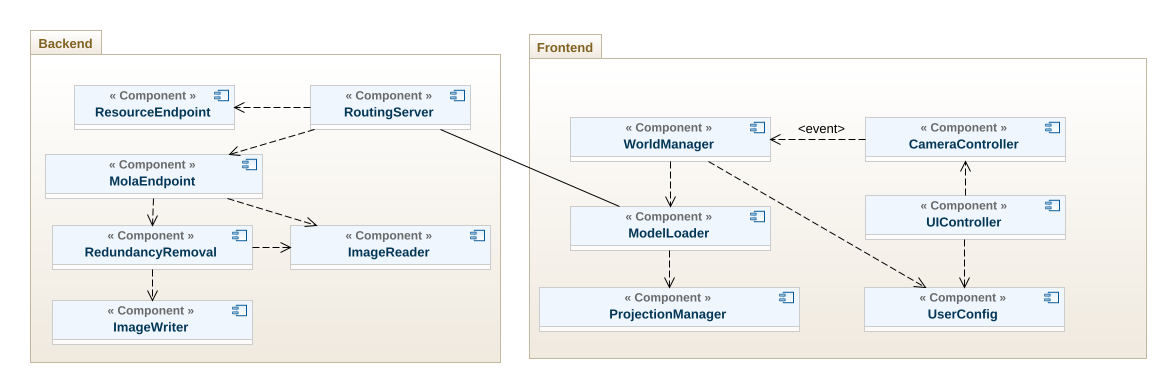
\includegraphics[width=\textwidth,keepaspectratio]{architectureOverview.png}
  \caption{Komponentendiagramm der SolarViewer Architektur}
  \label{architectureOverview}
\end{figure}

Das Backend hat eine sehr einfache Struktur und besitzt einen einzigen Einsteigspunkt, den \textit{RoutingServer}. Er ist dafür verantwortlich die eingehenden Requests an Hand ihrer URLs den einzelnen Endpoints zuzuordnen. Diese könnten in der Theorie auf verschiedenen Servern angesiedelt sein um ein Load Balancing zu ermöglichen. Dies ist für den Prototyp jedoch nicht erforderlich. Der \textit{ResourceEndpoint} ist dafür zuständig, alle statischen Resourcen wie die HTML-, CSS- oder JS-Dateien auszuliefern und bekommt alle Requests delegiert, welche vom RoutingServer keinem anderen Endpoint zugewiesen werden können. Der \textit{MolaEndpoint} ist für die Auslieferung der MOLA Daten zuständig. Er muss unter anderem die Dimensionen des zu ladenden Abschnitts übergeben bekommen und muss diesen Ausschnitt dann vom Dateisystem laden. Er ist des weiteren auf eine Komponente angewiesen, welche den Datensatz, wie in Abschnitt \ref{redundanzberechnung} beschrieben, von Redundanzen befreit. Diese Komponente muss dann in der Lage sein, die Daten wieder in das ursprüngliche Format zu schreiben, wofür die \textit{ImageWriter} Komponente zuständig sein soll. Die modifizierten Daten können dann abschließend mit dem \textit{ImageReader} gelesen und an das Frontend zurückgeliefert werden.

Das Frontend versucht durch eine lose Kopplung über Events die UI von der Logik zu trennen und orientiert sich am MVC-Pattern. Jegliche Aktionen des Benutzer, zum Beispiel ein Klick auf einen bestimmten Button, laden als erstes im \textit{UIController}. Er ist für die UI-Logik, unter anderem auch die Validation von User Eingaben, zuständig und schreibt alle benutzerspezifischen Konfigurationen in die \textit{UserConfig} Komponente. Diese Komponente besitzt keine Logik und kann direkt von anderen Komponenten genutzt werden um ihre Aufgaben zu spezifizieren. Der \textit{CameraController} bekommt alle Benutzeraktionen weitergeleitet, die von der UI nicht interpretiert werden konnten. Diese werden dann genutzt, um die Kamera zu bewegen oder zu rotieren. Diese Aktionen sorgen dann für die Generierung eines Events, welche das Laden der einzelnen Abschnitte initiiert. Verantwortlich dafür ist der \textit{WorldManager}. Er berechnet die Abchnitte die ge- oder entladen werden müssen, kümmert sich um den Detailgrad der Abschnitte und koordiniert den Ladevorgang. Auch besitzt er natürlich eine interne Repräsentation der aktuellen Abschnitte. Für das eigentliche Generieren eines Abschnitts ist dann der \textit{ModelLoader} zuständig. Er fragt den Server über einen HTTP Aufruf nach den Höhendaten und generiert daraus ein 3D Modell. Dabei nutzt er den \textit{ProjectionManager}, welche die Werte in verschiedene Projektion transformieren kann.

In Abbildung \ref{worldBuildingActivity} ist ein Aktivitätsdiagramm dargestellt, welches den geplanten Ablauf der Welterstellung auf Client-Seite grob darstellt. Die Aktivität wird durch jede Veränderung der Kamera durch den Benutzer gestartet. Dazu zählt die Translation durch die Benutzung der Pfeiltasten, die Rotation durch die Benutzung der Maus und die Skalierung oder Zoom durch die Benutzung des Mausrads.

\begin{figure}[H]
  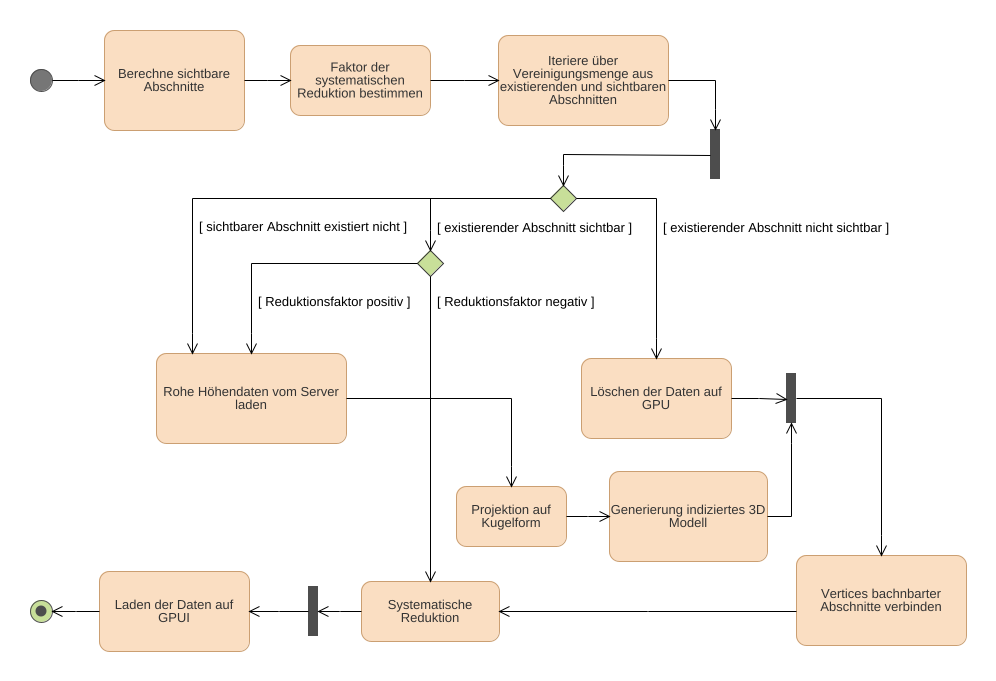
\includegraphics[width=\textwidth,keepaspectratio]{worldBuildingActivity.png}
  \caption{Aktivitätsdiagramm für die Erstellung der Welt auf Client-Seite}
  \label{worldBuildingActivity}
\end{figure}

Als erstes muss eine Liste aller sichtbaren Abschnitte angelegt werden. Dabei kommt das beschriebene frustum- und occlusion culling zur Anwendung. Da eine verlustfreie Reduktion der Datenmenge nicht ausreicht, muss eine systematische Reduktion stattfinden. Wie der Faktor schlussendlich berechnet wird, muss noch evaluiert werden, allerdings muss er von der Anzahl der sichtbaren Abschnitte abhängen und die Datenmenge auf einem möglichst konstanten Niveau halten. Als nächstes muss über die Vereinigungsmenge aller aktuell existierender und sichtbarer Abschnitte iteriert werden. Sollte der Abschnitt aktuell existieren, aber nicht mehr sichtbar sein, so muss er entladen werden. Hierbei ist darauf zu achten, auch die Ressourcen auf GPU Seite frei zu stellen, da dies natürlich nicht durch die automatische garbage collection auf JavaScript Seite abgedeckt ist. Sollte der Abschnitt aktuell existieren und auch weiterhin sichtbar sein, so muss geschaut werden, ob der Abschnitt aktuell den gleichen Reduktionsfaktor besitzt wie der berechnete. Ist dies der Fall, muss an dem Abschnitt nichts verändert werden. Sollte er größer sein, als der aktuelle Faktor, dann kann die Reduktion auf Client-Seite stattfinden, da nur eine eine bestimmte Anzahl an Vertices entfernt werden muss. Sollte er jedoch kleiner sein, so müssen die Daten erneut vom Server angefragt werden, da die Rohdaten natürlich nicht mit dem Modell gespeichert werden. Auch hierbei muss darauf geachtet werden, die aktuellen Daten zu löschen, sobald der neue Abschnitt vollständig geladen wurde. Hier muss geschaut werden, dass keine Ladeartefakte beim Tauschen des Abschnitts auftreten. Der letzte Fall in der Ladeschleife ist, dass ein sichtbarer Abschnitt nicht existiert. Hier muss dann wie beschrieben als erstes der Server nach den Daten gefragt werden. Da Netzwerkoperationen in der Regel immer relativ lange dauern, ist hier eine Parallelisierung geplant. Dies ist möglich, da in den nachfolgenden Aktionen keine Interaktion mit OpenGL notwendig ist. Als nächstes müssen die Daten in eine Kugelform projiziert werden, sollte dies vom Benutzer gewünscht werden. Auch muss aus den 1D Höhendaten jetzt ein vollständig indiziertes 3D Modell erzeugt werden. Ein Problem, dass bei der Benutzung von Abschnitten mit unterschiedlichen Modellen auftritt ist, dass diese eigentlich keine Vertices teilen. Die Polygone am Rand eines Abschnitts enden und verbinden sich nicht mit den Vertices des nächsten Abschnitts. Dies führt dazu, dass benachbarte Abschnitte eine sichtbare Lücke zwischeneinander besitzen. Um dies zu reparieren, muss als erstes darauf gewartet werden, dass alle parallel ladende Abschnitte fertig geladen wurden. Auch das Löschen muss zu diesem Zeitpunkt fertig sein, da klar sein muss, welcher Abschnitt welche Nachbarn besitzt. Dann müssen die Vertices der Kanten aller benachbarten Abschnitte in den eigenen Abschnitt kopiert werden. Erst wenn die Vertices eines Abschnitts vollständig definiert sind, kann die systematische Reduktion mit dem berechneten Faktor durchgeführt werden. Sobald dieser Ladevorgang für alle Abschnitte durchlaufen wurde, müssen die Daten erneut auf die GPU geladen werden. Hier ist erneut eine Synchronisation notwendig, da alle Befehle an OpenGL immer von einem Thread erfolgen müssen. Dies ist in der Regel der Thread, welcher den Grafikkontext initial angelegt hat. Man kann diesen Kontext zwar auch zwischen Threads wechseln, allerdings ist dies einer der teuersten Operationen in OpenGL und würde die Vorteile der Parallelisierung zunichte machen. Ob dies im Kontext von WebWorkern eines Browsers überhaupt funktioniert, ist auch fragwürdig, da diese in der Regel keinen Zugriff auf das DOM und somit auf die Canvas besitzen.

\section{User Interface}
Im Laufe der Planungsphase wurde anschließend ein Mock Up angelegt, welches in Abbildung \ref{mockUp} betrachtet werden kann. Wichtig beim Design war, das nur das grundlegende Konzept geplant werden soll und spezielle Details außen vor gelassen werden. Diese können dann während der Implementierungsphase evaluiert werden. Dies ist zum einen dem Grund geschuldet, dass einige Unsicherheiten darin bestehen, welche Informationen der Implementation vom Benutzer zur Verfügung gestellt werden müssen. Zum anderen gibt es einige fakultative Anforderungen, bei denen noch nicht klar ist, ob sie schlussendlich umgesetzt werden.

\begin{figure}[H]
  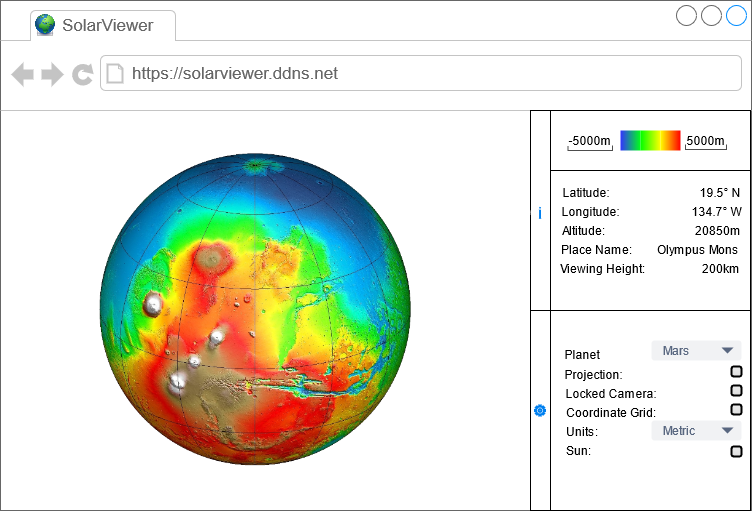
\includegraphics[width=\textwidth,keepaspectratio]{mockUp.png}
  \caption{Mock Up der SolarViewer Anwendung}
  \label{mockUp}
\end{figure}

Das Design orientiert grundsätzlich sich an den analysierten Visualisierungen (siehe \ref{istZustand}). Dabei soll die Visualisierung im Mittelpunk stehen und eine kleine UI die Navigation unterstützen und einige nützliche Informationen anzeigen. Das Hauptkriterium für die UI ist der Ansatz, dass sie die Visualisierung in keinster Weise beeinträchtigen darf. Der User soll selbst entscheiden können, welche Informationen er benötigt. Dies soll über ausfahrbare Panels realisiert werden, die von einer Seite der Anwendung ein- und ausgeblendet werden können. Dabei sollen die unterschiedlichen Panels unabhängig voneinander agieren können und möglichst ähnliche Arten von Informationen beinhalten. Fürs erste soll die UI daher in mindestens drei Bereiche gegliedert werden: Visualisierung, Informationen und Konfigurationen. Hier könnte eine Aufteilung in weitere Panels, potentiell auf der anderen Seite der UI, sinnvoll sein, je nachdem welche Anforderungen umgesetzt werden können. Alle Panels sollen über ein kleines, deskriptives Icon am Rand identifiziert werden können. Hier wurde sich an gängigen Icons orientiert und ein Zahnrad für die Konfiguration und das bekannte Informationsicon für den Informationsbereich entschieden. Die Panels sollen initial eingeklappt sein um dem User die Dimensionen der Buttons zum Öffnen der Panels zu vermitteln. Ein Klick auf die eigentlichen Panels soll keinen Effekt haben, um versehentliches Schließen der Panels zu verhindern.

Das Informationspanel soll als erstes eine Skala zeigen, die die verwendeten Farben einem Höhenwert zuordnet. Da dies natürlich eine zentrale Information ist, ohne die die Visualisierung nicht verstanden werden kann, wurde als Alternative überlegt, sie dauerhaft im Hauptteil anzeigen zu lassen. Damit würden dem Benutzer einige unnötige Klicks erspart werden, allerdings steht es im Widerspruch zum Kernkriterium, dass die Visualisierung nicht eingeschränkt werden darf. Bei besonders hohen Zoomstufen würde sich die Skala unweigerlich mit der Visualisierung überlagern und dies soll vermieden werden. Auch könnte der Nutzer diese Information dann nicht ausblenden, was ein Kernaspekt des Designs ist. Hier ist eine weitere Nutzer-Evaluation notwendig um dies zu bestätigen. Ein weiteres Problem ist die Schwierigkeit den Farben jetzt Höhenwerten zuzuordnen. Idealerweise muss dem Nutzer auf einen Blick klar sein, welche Farbe zu welchem Höhenwert gehört. Es ist jedoch aus Platzgründen schwer, mehrere Höhenangaben in die Skala aufzunehmen. Es wurde also entschieden, nur den minimalen und maximalen Höhenwert an den Rändern anzuzeigen. Hier muss vorausgesetzt werden, dass der Nutzer die Linearität versteht und sich die Höhenwerte zwischen den Grenzen erschließen kann. Auch dies muss im weiteren Verlauf mit Test-Nutzern evaluiert werden. Die Grenzen sollen laut den Anforderungen auch änderbar sein, daher muss dem Nutzer dies auch signalisiert werden. Hier wurde sich für ein Design ähnlich dem von Links entschieden, das zu einem Klick auf die Zahlen einladen soll.

Weitere Informationen auf dem Panel sollen die Koordinaten, die Höhenangabe und potentiell der Name des Ortes sein. Im Gegensatz zu den restlichen Informationen hängt es davon ab, auf welche Stelle der Nutzer auf dem Globus klickt. Hier wurde schon im voraus die fehlende Erklärung als Problem identifiziert. Es gibt kein Hinweis, der den Nutzer zu einem Klick auf den Globus verleitet. Sollte er als erstes das Informationspanel öffnen, so würden dort keine Informationen angezeigt werden können und der Nutzer könnte dies als Fehler werten. Auch ist unklar, was bei Klicks neben den Globus passieren sollte. Eine Möglichkeit wäre es, den Mauscursor zu einem bekannten, zu einem Klick verleitenden Cursor zu verändern, solange er sich über dem Globus befindet. Des Weiteren könnte man an Stelle von leeren Werte eine Textnachricht anzeigen, die den Nutzer zum Klick auf den Globus auffordert. Eine sehr gute Alternative nutzt die Google Earth Anwendung. Bei ihr kann man einen kleinen Marker per Drag\&Drop an eine bestimmte Stelle ziehen, was sehr intuitiv ist, aber gleichzeitig wohl auch zu komplex für diese Anwendung. Im Endeffekt wird wohl auch Zeitgründen eine Textnachricht zum Einsatz kommen müssen, auch wenn Text aus Gründen der User Experience immer vermieden werden sollte. Des Weiteren soll noch die Höhe des Betrachters über der Erdoberfläche angezeigt werden, dies erfordert allerdings keine besonderen Nutzerinteraktionen und stellt daher kein Problem dar. Eine Designentscheidung bei all diesen Werten ist die Genauigkeit der angezeigten Werte. Dies ist natürlich abhängig von der schlussendlichen Nutzung der Anwendung und kann zwischen wissenschaftlicher und privater Nutzung stark schwanken. Idealerweise sollte die Genauigkeit deshalb konfigurierbar sein. Als Standard wurde hier eine eher geringere Genauigkeit gewählt, die allerdings abhängig von dem verwendeten Wert ist. Der Werte der Betrachterhöhe sollte auf Kilometer, die Erdbodenhöhe auf Meter und die Koordinaten auf eine Nachkommastelle gerundet werden.

Das Konfigurationspanel soll als erstes eine Möglichkeit beinhalten, den angezeigten Datensatz, bzw. den Planeten, zu ändern. Auch wenn die Anwendung fürs erste nur den Mars visualisieren soll, soll der Visualisierung weiterer Planeten nichts im Wege stehen und dies muss schon bei der ursprünglichen UI Gestaltung beachtet werden. Des Weiteren soll der Nutzer die Projektion ein- und ausschalten können. Andere Alternativen nutzen hier noch komplexere Auswahlmöglichkeiten (z.B. unterschiedliche Kugelprojektion oder Projektionen der Pole), dies soll mit einer reinen Checkbox allerdings vereinfacht werden. Auch muss laut Anforderungen die Möglichkeit geschaffen werden, zwischen einer statischen und frei beweglichen Kamera zu wechseln. Ob hier ein besserer Weg gefunden werden kann, idealerweise ohne jedes Mal die Konfiguration zu öffnen, muss im Projektverlauf überlegt werden. Des Weiteren soll der Benutzer die Möglichkeit besitzen, die Einheiten der Höhenwerte zu ändern. Dabei soll zumindest die Wahl zwischen metrischen und imperialen ermöglicht werden. Falls im Projektverlauf keine weiteren Messsysteme gefunden werden können, kann dies auch als Checkbox realisiert werden. Des Weiteren sind in dem Panel weitere Optionen möglich, im konkreten Fall wurde Optionen zum ein- und ausschalten eines realistischen Beleuchtungsmodells und der Koordinatenlinien erdacht. Dies hängt natürlich stark von den schlussendlich implementierten Funktionen ab. Falls das Hinzufügen von Optionen aus Platzgründen schwierig wird, so muss das Informationspanel auf die andere Seite der Fensters verschoben werden.

Die Sprache der Anwendung soll Englisch sein, da so wieder die größere Zielgruppe erreicht werden kann. Insbesondere im akademischen Bereich und im Bereich der Raumfahrt sollte dies auch kein Problem darstellen, da hier Englischkenntnisse weit verbreitet sind. Die Wahl des Logos ist noch nicht final, es soll etwas universelles darstellen, was die Leute mit verschiedenen Planeten des Sonnensystems, nicht nur mit einem Planten, in Verbindung bringen. Fürs erste wurde dafür ein kleines Erdlogo geplant. Für die Icons soll der Anbieter FontAwesome genutzt werden. Er stellt in einer freien Lizenz über 1600 verschiedene Icons bereit, welche als CSS Datei, gehosted auf FontAwesome Servern, in die Webseite eingebunden werden. Konkrete Icons können dann über CSS Klassen definiert werden, wobei für jedes Icon auch verschiedene Variationen bereitgestellt werden (solide, leichtgewichtig, mehrfarbig, etc.). Auch die Größen lassen sich ohne Verlust der Auflösung stark variieren und die Farben sind frei wählbar.